%===================================================================================
% JORNADA CIENTÍFICA ESTUDIANTIL - MATCOM, UH
%===================================================================================
% Esta plantilla ha sido diseñada para ser usada en los artículos de la
% Jornada Científica Estudiantil de MatCom.
%
% Por favor, siga las instrucciones de esta plantilla y rellene en las secciones
% correspondientes.
%
% NOTA: Necesitará el archivo 'jcematcom.sty' en la misma carpeta donde esté este
%       archivo para poder utilizar esta plantila.
%===================================================================================



%===================================================================================
% PREÁMBULO
%-----------------------------------------------------------------------------------
\documentclass[a4paper,10pt,twocolumn]{article}

%===================================================================================
% Paquetes
%-----------------------------------------------------------------------------------
\usepackage{amsmath}
\usepackage{todonotes}
\usepackage{amsfonts}
\usepackage{amssymb}
\usepackage{jcematcom}
\usepackage[utf8]{inputenc}
\usepackage{listings}
\usepackage[pdftex]{hyperref}
\usepackage{caption}
\usepackage{subcaption}
\usepackage{siunitx}
%-----------------------------------------------------------------------------------
% Configuración
%-----------------------------------------------------------------------------------
\hypersetup{colorlinks,%
	    citecolor=black,%
	    filecolor=black,%
	    linkcolor=black,%
	    urlcolor=blue}

%===================================================================================



%===================================================================================
% Presentacion
%-----------------------------------------------------------------------------------
% Título
%-----------------------------------------------------------------------------------
\title{Diferencias en diferencias. Estudio: Meningitis en Cuba}

%-----------------------------------------------------------------------------------
% Autores
%-----------------------------------------------------------------------------------
\author{\\
\name Jackson Vera Pineda \email \href{mailto:jacksonverapineda@gmail.com}{jacksonverapineda@gmail.com}
	\\ \addr Grupo C312 
  }

%-----------------------------------------------------------------------------------
% Tutores
%-----------------------------------------------------------------------------------
\tutors{\\
%Dr. José E. Valdez Castro, \emph{Universidad de la Habana.} \\
%MsC. Yanetsy E. Rodríguez, \emph{Universidad de la Habana.} \\
}

%-----------------------------------------------------------------------------------
% Headings
%-----------------------------------------------------------------------------------
\jcematcomheading{\the\year}{1-\pageref{end}}{Vera J.}

%-----------------------------------------------------------------------------------
\ShortHeadings{Diferencias en diferencias - Meningitis en Cuba}{Autores}
%===================================================================================



%===================================================================================
% DOCUMENTO
%-----------------------------------------------------------------------------------
\begin{document}

%-----------------------------------------------------------------------------------
% NO BORRAR ESTA LINEA!
%-----------------------------------------------------------------------------------
\twocolumn[
%-----------------------------------------------------------------------------------

\maketitle

%===================================================================================
% Resumen y Abstract
%-----------------------------------------------------------------------------------
\selectlanguage{spanish} % Para producir el documento en Español

%-----------------------------------------------------------------------------------
% Resumen en Español
%-----------------------------------------------------------------------------------
%\begin{abstract}
%
%	El resumen en español debe constar de $100$ a $200$ palabras y presentar de forma
%	clara y concisa el contenido fundamental del artículo.
%
%\end{abstract}
%
%%-----------------------------------------------------------------------------------
%% English Abstract
%%-----------------------------------------------------------------------------------
%\vspace{0.5cm}
%
%\begin{enabstract}
%
%  The English abstract must have have $100$ to $200$ words, and present 
%  the essentials of the article content in a clear and concise form.
%
%\end{enabstract}

%-----------------------------------------------------------------------------------
% Palabras clave
%-----------------------------------------------------------------------------------
\begin{keywords}
	estadística,
	bioestadistica,
	inferencia causal,
	diferencias en diferencias,
	cuasiexperimento.
\end{keywords}

%-----------------------------------------------------------------------------------
% Temas
%-----------------------------------------------------------------------------------
\begin{topics}
	Estadística, Salud Pública, Biomatemática
\end{topics}


%-----------------------------------------------------------------------------------
% NO BORRAR ESTAS LINEAS!
%-----------------------------------------------------------------------------------
\vspace{0.8cm}
]
%-----------------------------------------------------------------------------------


%===================================================================================

%===================================================================================
% Introducción
%-----------------------------------------------------------------------------------
\section{Introducción}\label{sec:intro}
%-----------------------------------------------------------------------------------
		La meningitis es la inflamación de los tejidos que rodean el cerebro y la médula espinal, generalmente causada por una infección. Puede ser mortal y requiere atención médica inmediata. Diversas especies de bacterias, virus, hongos y parásitos pueden provocarla, siendo la meningitis bacteriana la más peligrosa, con potencial de causar la muerte en menos de 24 horas y afectando a personas de cualquier edad \cite{OMS_meinigitis}. Desde su identificación por Gaspard Vieusseux en 1805, el término ha sido utilizado para describir brotes y epidemias en diferentes regiones del mundo.A finales del siglo XIX se descubrien bacterias causantes de la Enfermedad Meningocócica: S. pneumoniae por Louis Pasteur (Francia) y George Sternberg (Estados Unidos de América, simultaneamente en 1880; Neisseria meningitidis en 1887 por el patólogo austriaco Antón Weichselbaum; y más tarde en 1892, se identifica H. influenzae por Richard Pfeiffer en Alemania.  \cite{batlle}. Durante el siglo XX, la meningitis mostró un aumento en la frecuencia de casos y epidemias, con cifras de letalidad cercanas al 100\%. A pesar de los intentos iniciales de tratamiento con antisueros, fue la introducción de antibióticos como la penicilina en la década de 1940 lo que permitió cambios favorables en la morbilidad y mortalidad asociadas a estas infecciones.
		
		En Cuba, la recolección de datos históricos sobre la Meningitis de fuentes confiables, en la etapa colonial, ha sido complicada debido a la pérdida de registros y la falta de precisión en los diagnósticos (muchas epidemias eran denominadas "peste", independeiente de su causa). Hasta el momento, la referencia más antigua a la enfermandad en la mayor de las Antillas, en un documento científico de fuente confiable, fue encontrada en los Anales de la Real Academia de Ciencias Físicas y Naturales de La Habana. En uno de ellos, el Dr. González del Valle describe que, durante el invierno y la primavera de 1877, hubo 148 fallecidos por meningitis que constituyeron el 3,7 \% de todas las muertes ocurridas en ese año.  \cite{batlle}
		
		El libro Enfermedad Meningocócica: cronología de una Epidemia donde Valcárcel et al., revela un brote epidémico en esa misma La Habana en 1921 y algunos casos en el país en 1925, así como otros pasajes de la enfermadad en la Neocolonia.  \cite{valcarcel}
		
		Entre 1959 y 1974, Cuba reportó pocos casos anuales de meningitis, pero en 1976, se inicia una epidemia a partir de un brote ocurrido en el área de salud del Policlínico “26 de Julio” de Ciudad de La Habana, donde se diagnostican seis casos, de los cuales tres fallecen y tres se confirman bacteriológicamente. A partir entonces, se observa un incremento de la incidencia de la enfermedad causada principalmente por N. meningitidis del serogrupo C. Por esta razón, en 1979, el Ministerio de Salud Pública (Minsap) decide aplicar la vacuna anti-meningocócica polisacarídica A-C (Pasteur-Mérieux®, Francia) se observa una disminución considerable de la proporción de casos causados por el serogrupo C. A pesar de esto, la incidencia continúa en ascenso y alcanza cifras epidémicas, pero ahora ocasionada por el serogrupo B.  \cite{batlle}
		
		Ante la ausencia de una vacuna efectiva contra el serogrupo B, se inicia el desarrollo y la obtención de una vacuna cubana antimeningocócica contra este serogrupo a partir de 1984. Una vez obtenido en el Instituto Finlay de La Habana el preparado vacunal VA-MENGOC BC®, que demostró gran seguridad y efectividad contra los serogrupos B y C, que se usa masivamente (1987) y se contribuye al control, incluyéndose en el Programa Nacional de Inmunizaciones (1991) \cite{batlle}
		
		El efecto causal de politicas y programas relacionados con vacunas, seguridad, sustancias tóxicas, contaminación, drogas legales e ilegales, y comportamientos de salud es difícil de medir; pero el desarrollo social exige conocimiento acerca de relaciones causales. El consejo estándar es implementar un ensayo controlado aleatorio (RCT)  \footnote{ en ingles \emph{Randomized Controlled Trials} (RCT), los Ensayos Controlados Aleatorios describen los estudios experimentales en los que los participantes son asignados de manera aleatoria a diferentes grupos, generalmente un grupo de tratamiento y un grupo de control, con el objetivo de evaluar la eficacia de una intervención o tratamiento específico.} para evitar confusiones y aislar los efectos del tratamiento. Pero los RCT a gran escala son raros en la práctica. Diferencias en Diferencias (DD) es un diseño cuasiexperimental de investigación que generalmente es usado para estudiar relaciones causales, a pesar de sus limitaciones, cuando la realización de Ensayos Controlados Aleatorios es imposible o inmoral. \cite{wing}
		
		En el presente estudio, se propone realizar un análisis del impacto de la vacuna cubana VA-MENGOC BC® en el país caribeño, tras su aplicación masiva en 1987. Usando el método de Diferencias en Diferencias con datos hístoricos de la mortalidad Cuba por Meningitis (como grupo de tratamiento) y otras dos causas (como grupo de control) evaluaremos la eficacia de la vacuna como factor causal de la disminución del número de fallecidos por la enfermedad durante el periodo de 1980 hasta el 2000.
		

%===================================================================================
%En un estudio que incluyó a 5,742 niños, se concluyo que el promedio de Longitud Axial (AL) era de 23.7 mm (rango: 18.3 mm a 30.4 mm).


%===================================================================================
% Desarrollo
%-----------------------------------------------------------------------------------
\section{Desarrollo}\label{sec:dev}
%-----------------------------------------------------------------------------------
%  En esta sección (o secciones) incluya el contenido fundamental del artículo.
%  No es necesario tener una sección nombrada \emph{Desarrollo}, por el contrario,
%  nombre las secciones según el contenido que tratan.
	  \subsection{Sobre los datos}\label{sub:data}
  
%	Los datos fueron obtenidos de Kaggle \cite{kaggle}. Las mediciones se realizaron al ojo derecho de cada individuo por tanto, cada observación está asociada a un sujeto independiente. Como denota del nombre OLSM, el estudio fue de forma longitudinal, es decir, se realizó un seguimiento a cada sujeto del estudio por varios años \footnote{ La alternativa más común a estudio transversal, lo que significa que captura una instantánea de un grupo en un momento específico. Un estudio longitudinal observa a un grupo repetidamente a lo largo de un período de tiempo. \cite{downey}}, y en el conjunto actual se presenta la última revisión, como se especifica en el artículo por Zadnik K. \cite{zadnikpredictors}
  
% 	\begin{figure*}[ht!]%
%  		\begin{center}
%	  		\begin{tabular}{lS[table-format=3.2]@{\space$\, \pm \,$}S[table-format=2.2]SS}
%	  			\hline
%	  			\multicolumn{1}{c}{\textbf{Variables}} & \multicolumn{2}{c}{\textbf{Media $\pm$ SD}} & \multicolumn{1}{c}{\textbf{Mínimo}} & \multicolumn{1}{c}{\textbf{Máximo}}\\
%	  			\hline
%	  			Edad & 6.30 & 0.71	& 5 & 9 \\ 
%	  			Equivalente Esférico de Refracción (D)	& 0.80 & 0.63 & -0.70 & 4.37 \\ 
%	  			Longitud Axial (mm) & 22.50 & 0.68 & 19.90 & 24.56 \\ 
%	  			Profundidad de la Cámara Anterior (mm) & 3.58 &  0.23 & 2.77 & 4.25 \\ 
%%	  			Grosor del Critalino & 3.54	& 0.15 & 2.96 &	4.11 \\ 
%	  			Produndidad de la Cámara Vítrea (mm) & 15.38	& 0.66 & 13.38 & 17.30 \\ 
%%	  			Tiempo al aire libre &	11.95 & 7.97 & 0 & 45 \\ 
%%	  			Tiempo de Lectura recreativa & 2.80 & 3.07 & 0 & 20 \\
%%	  			Tiempo en Computadora & 2.10 & 3.05 & 0 & 30 \\
%%	  			Tiempo de estudio & 1.49 & 2.22 & 0 & 15 \\
%%	  			Tiempo viendo televisión & 8.95 & 5.72 & 0 & 31 \\
%%	  			Compuesto de act & 22.01 & 26.03 & 2 & 101 \\ 
%	  			\hline
%	  		\end{tabular}
%  			\caption{ Resumen descriptivo de las variables numéricas.\label{table:1}}
%  	\end{center}
%  \end{figure*}
%  
%  \subsection{Variables}\label{sub:variables}
%  	  A continuacion se presentan las variables del conjunto de datos más relevantes para el presente análisis, y, en la Tabla \ref{table:1}, se expone un resumen descriptivo de cada una en la muestra :
%  	\begin{description}
%  
%%  	\item \texttt{STUDYYEAR}: Año en el que se realizó la medición.
%  	\item [\texttt{MYOPIC}]: Variable booleana 0 si el sujeto desarrollara miopía en los siguientes 5 años o no
%  	\item [\texttt{AGE}]: La Edad del sujeto (de 5 a 9 años)
%  	\item [\texttt{GENDER}]: Género del sujeto 1 Femenino 0 Masculino,
%  	\item [\texttt{SPHEQ}]: Equivalente Esférico de la Refracción ( Spherical Equivalent Refraction) es una estimación del error refractivo de los ojos (Medición en D, dioptría).
%  	\item [\texttt{AL}]: La Longitud Axial se refiere a la distancia entre la parte posterior y la parte delantera del ojo   (Medición en milímetros mm).
%%  	\item [\texttt{ACD}]: La Profundidad de la Cámara Anterior (Anterior Chamber Depth) se refiere a la distancia entre la superficie anterior de la córnea y la superficie anterior del cristalino (Medición en milímetros).
%%  	\item [\texttt{LT}]: El grosor del cristalino (Medición en milímetros mm) rango de 20.48-35.05 mm.
%%  	Cambios con la Longitud Axial (AL): El LT no cambia de manera lineal con la AL. En ojos cortos, el LT aumenta a medida que la AL aumenta. Sin embargo, en ojos normales o moderadamente miopes, disminuye con una AL más larga. Curiosamente, en ojos altamente miopes, vuelve a aumentar con una AL mayor. El LT máximo se encuentra en el grupo de AL de 20.01–22 mm.
%%  	El LT se correlaciona negativamente con la ACD.
%  	\item [\texttt{VCD}]: La Profundidad de la Cámara Vítrea (Vitreous Chamber Depth, en inglés) en oftalmología se refiere a la distancia entre la parte posterior del cristalino y la retina.
%%  	En pacientes en edad pediátrica existe una correlacion débil directa, pero no puede asegurarse puesto que puede depender de otros factores.
%%  	\item [\texttt{SPORTHR}]: Tiempo de Recreación al aire libre (Horas por Semana)
%%	\item [\texttt{READHR}]: Tiempo de Lectura recreativa (Horas por Semana)
%%  	\item [\texttt{COMPHR}]: Tiempo Activo en Computadora o consolas (Horas por Semana).
%% 	\item [\texttt{STUDYHR}]: Tiempo de estudio (Horas por Semana).
%%  	\item [\texttt{TVHR}]: Tiempo viendo televisión (Horas por Semana).
%%  	\item [\texttt{DIOPTERHR}]: Compuesto de actividades cercanas al trabajo (horas/semana).
%  	\item [\texttt{MOMMY}]: Se refiere a si la madre es miope 0 negativo, 1 positivo.
%  	\item [\texttt{DADMY}]: Se refiere a si el padre es miope 0 negativo, 1 positivo.
%  	
%  	%
%  \end{description}
%  
%  
%
%  
%
%%%-----------------------------------------------------------------------------------
%%	\subsection{Organización del Documento}\label{sub:results}
%%%-----------------------------------------------------------------------------------
%%		Puede agregar secciones y subsecciones según sea necesario para organizar
%%		de manera más coherente su artículo. Tenga en cuenta que un documento más
%%		plano es más fácil de navegar y entender, pero las subsecciones relacionadas
%%		deberían estar agrupadas en una sección común.
%%		
%%		
%%		Los nombres de las secciones deben ir en mayúsculas, excepto para las
%%		preposiciones, conjunciones, y otros vocablos auxiliares.
%%
%%		Empiece un nuevo párrafo cada vez que vaya a comenzar una idea nueva.
%%		
%%-----------------------------------------------------------------------------------
%\subsection{Visualización de Datos}\label{sub:visualization}
%%-----------------------------------------------------------------------------------
%	Como puede observarse en la Figura \ref{fig:6a}, la cantidad de pacientes de género masculino y femenino está equilibrada (variable GENDER). Sin embargo no puede afirmarse lo mismo del número de pacientes miopes Figura \ref{fig:6b}, que es más de 6 veces menor que el número de pacientes sin la afección, este sesgo puede estar dado porque el comienzo de dicho problema con frecuencia se ubica entre los 6 y los 14 años, afecta aproximadamente al 5\% de los niños en edad preescolar, al 9\% de los niños en edad escolar \cite{oftalmolima}.
%	
%	\begin{figure}[htb]
%		\begin{subfigure}{.49\linewidth}
%			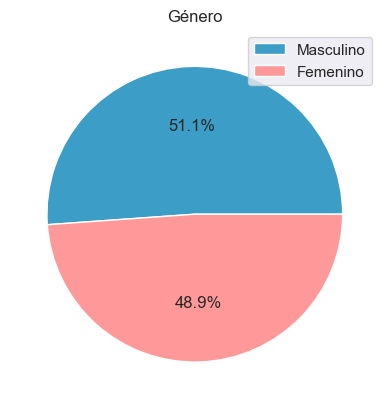
\includegraphics[height=.95\linewidth, width=.95\linewidth]{assets/GENDER_pie}
%			\caption{}
%			\label{fig:6a}
%		\end{subfigure}
%		\begin{subfigure}{.49\linewidth}
%			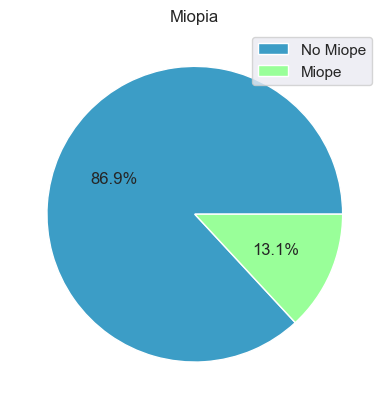
\includegraphics[height=.95\linewidth, width=.95\linewidth]{assets/MYOPIC_pie}
%			\caption{}
%			\label{fig:6b}
%		\end{subfigure}
%		\caption{Gráfico de Pastel, Género (a), y Miopía (b).}
%		\label{fig:6}
%	\end{figure}
%	
%	
%	\begin{figure}[htb]
%		\begin{subfigure}{.49\linewidth}
%			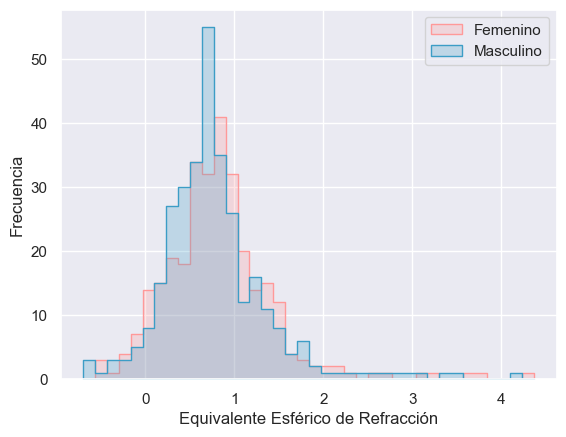
\includegraphics[height=.95\linewidth, width=.95\linewidth]{assets/SPHEQ_gender_hist}
%			\caption{}
%			\label{fig:7a}
%		\end{subfigure}
%		\begin{subfigure}{.49\linewidth}
%			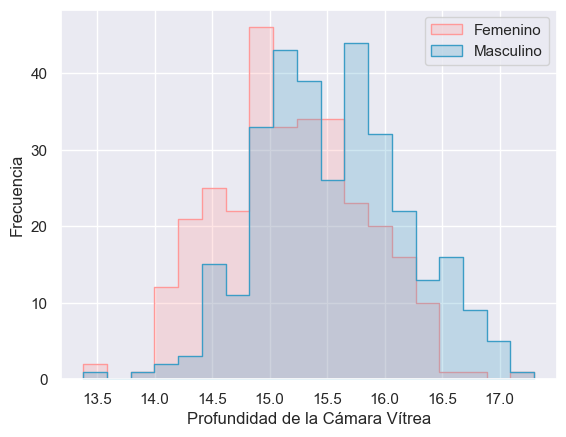
\includegraphics[height=.95\linewidth, width=.95\linewidth]{assets/VCD_gender_hist}
%			\caption{}
%			\label{fig:7b}
%		\end{subfigure}
%		    \vspace{\baselineskip}
%		\begin{subfigure}{\linewidth}
%			\centering
%			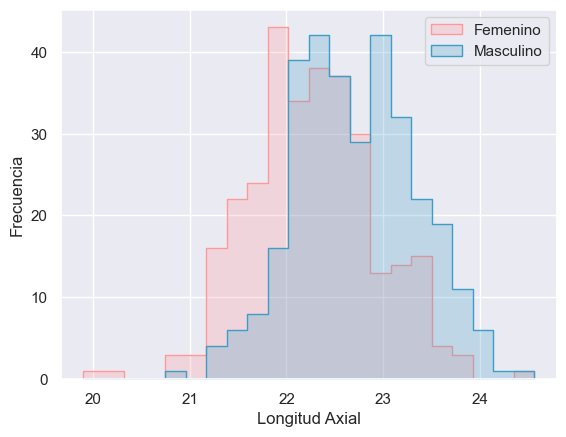
\includegraphics[height=.5\linewidth, width=.5\linewidth]{assets/AL_gender_hist}
%			\caption{}
%			\label{fig:7c}
%		\end{subfigure}
%		\caption{Histograma, SPHEQ (a),  VCD (b) y AL (c) según el género del paciente.}
%		\label{fig:7}
%	\end{figure}
%	
%	En la Figura  \ref{fig:7} se expone histogramas de las variables Equivalente Esférico de Refracción (SPHEQ) \ref{fig:7a} , Profundidad de la Cámara Vítrea (VCD) \ref{fig:7b} y la Longitud Axial (AL) \ref{fig:7c}, según el genero del paciente. Nótese que no se muestran diferencias importantes en las distribuciones y es que los infantes suelen tener características similares cuando son muy pequeños, pero después de los 9 años comienzan a diferenciarse mas por ejemplo: los niños tienden a mostrar longitudes axiales más largas que las niñas; los ojos asiáticos tienden a ser más largos que los ojos caucásicos.
%	\\
%	
%	El uso de datos de la AL es valioso tanto para determinar el riesgo para la salud ocular, como para juzgar la eficacia de un tratamiento para el control de la miopía. Varios estudios han demostrado la correlación entre la biometría ocular, especialmente la AL, con los errores refractivos: se encontró que el SPHEQ y la ACD afectaban los parámetros de la AL. Estas relaciones pueden distinguirse en la Figura \ref{fig:4}, que representa un gráfico por pares de las variables AL, SPHEQ y VCD, con histograma de estas variables en la diagonal.
%	
%	Cabe destacar en la Figura \ref{fig:4} cómo el SPHEQ a priori parece ser un elemento clave a tomar en cuenta en la predicción de la miopía, dado el posicionamiento de los pacientes convalecientes en los valores donde el SPHEQ es bajo. Además, es notoria la fuerte relación que existe entre  la AL y VCD, lo cual es intuitivo dado que la Cámara Vitréa constituye gran parte del globo ocular.
%	
%		\begin{figure}[ht]%
%		\begin{center}
%			\centering
%			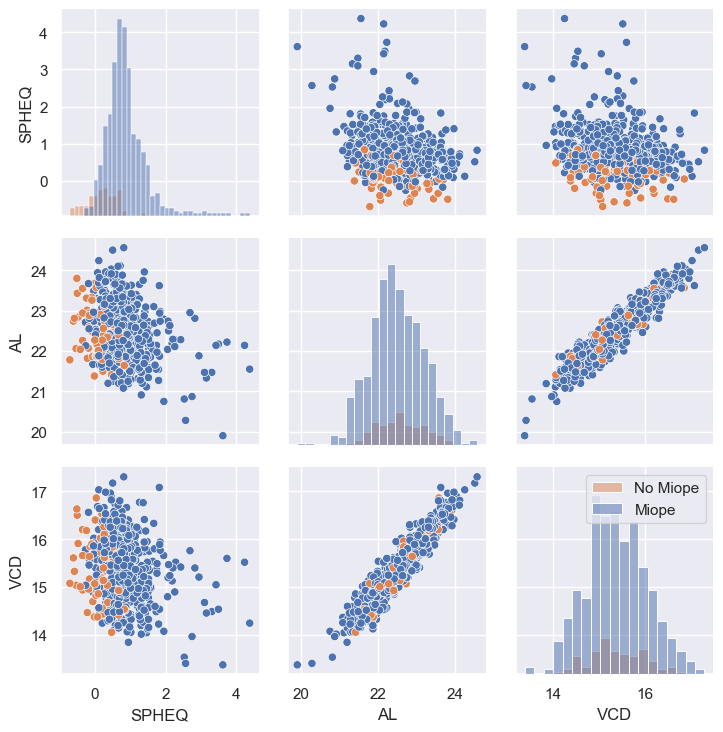
\includegraphics[height = .75\linewidth, width=.8\linewidth]{assets/focused_pairplot}
%		\end{center}
%		\caption{Gráfico por pares de las variables AL, VCD, SPHEQ, y la presencia de miopía (puntos en naranja).}
%		\label{fig:4}
%	\end{figure}
%	
%	%-----------------------------------------------------------------------------------
%	\subsection{Pruebas de Hipótesis}\label{sub:hiptesting}
%	%-----------------------------------------------------------------------------------
%	 
%	 En  la Figura \ref{fig:1} puede notarse que la Longitud Axial en los datos parece estar normalmente distribuida, de ahí que resulta ingteresante el  análisis  de esta variable para comprobar su normalidad, y conocer qué posibles propiedades cumple.
%
%	 \begin{figure}[htb]
%		\begin{subfigure}{.49\linewidth}
%			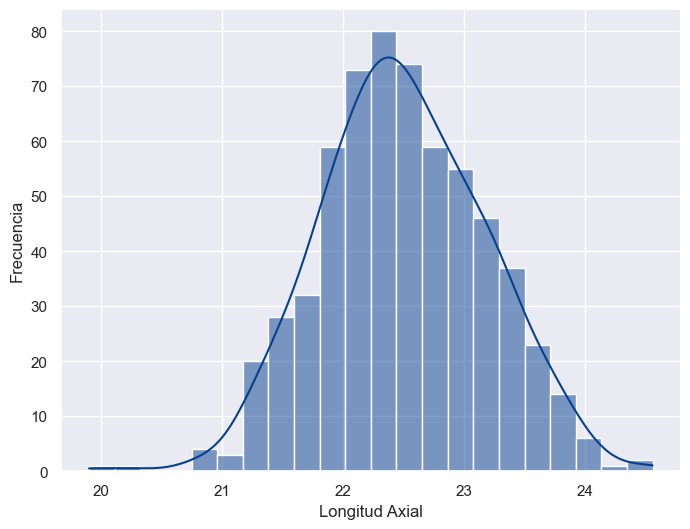
\includegraphics[height=.95\linewidth, width=.95\linewidth]{assets/AL_hist}
%			\caption{}
%			\label{fig:1a}
%		\end{subfigure}
%		\begin{subfigure}{.49\linewidth}
%			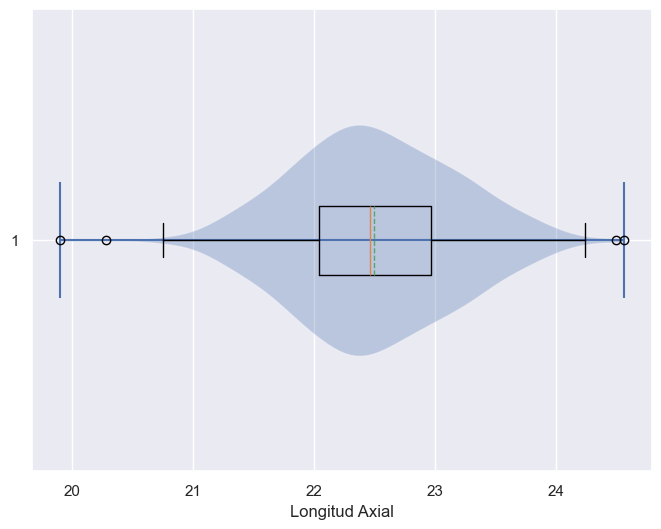
\includegraphics[height=.95\linewidth, width=.95\linewidth]{assets/AL_boxplot}
%			\caption{}
%			\label{fig:1b}
%		\end{subfigure}
%		\caption{La distribución de la Longitud Axial, representada en un histograma (a), y gráfico de cajas, bigotes, y violín (b).}
%		\label{fig:1}
%	\end{figure}
%	
%	Se procede a realizar un gráfico Cuantil-Cuantil como se muestra en la Figura \ref{fig:2}. Efectivamente, los cuantiles teóricos de una población normalmente distribuida coinciden con los cuantiles muestrales. Luego, se estiman la media y desviación estándar de la población ($\mu \approx 22.50$ y $\sigma \approx 0.69$), y se realiza una prueba de bondad de ajuste, Kolmogorov- Smirnov, entre la muestra y una población normal teórica construida con los parámetros estimados previamente; arrojando \emph{p-value} $ = 0.77 $, donde $\alpha$ es el nivel de significancia. Por tanto, no se tiene evidencia suficiente para rechazar  la normalidad de la Longitud Axial.
%	\\
%	
%		\begin{figure}[htb]%
%		\begin{center}
%			\centering
%			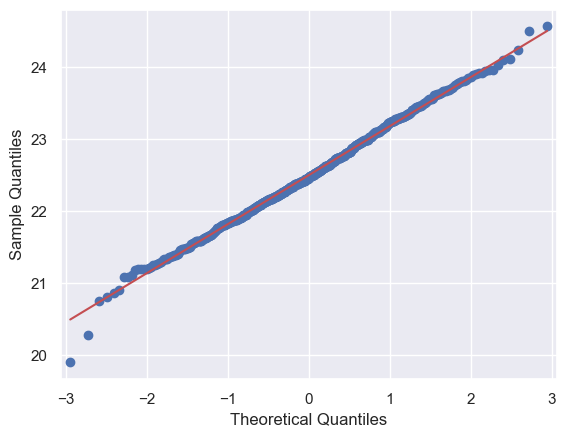
\includegraphics[height = .75\linewidth, width=.75\linewidth]{assets/AL_qqplot}
%		\end{center}
%		\caption{Gráfico Cuantil-Cuantil de la Longitud Axial, donde los cuantiles teóricos se refieren a una población normalmente distribuida.}
%		\label{fig:2}
%	\end{figure}
%	
%	 En 2021 He X., Sankaridurg P. y un colectivo de científicos analizaron la correlación entre la AL en diferentes grupos etarios y la aparición de miopía en un estudio transversal en China. Dicho estudio incluyó un total de $14127$ participantes (en su mayoría chinos), y de ellos 5742 niños entre 7 y 10 años \cite{hex}. Entre sus resultados determinaron la media de la AL, con un valor aproximado de $22.9$ ($\pm 0.8$ , desviación estándar) para un rango de edades similar al de la muestra bajo el presente análisis.
%	 
%	 De la estimación anteriormente calculada de la media muestral ($\bar{X} = 22.5 $). Luego, se comprueba mediante una prueba de hipótesis t-student si $H_0$: la media de la población de la que fue extraída la muestra coincide con la analizada por He X., $H_1$: la media de la población es menor. El resultado arrojó un $p-value = 1.22e-42$, por tanto se rechaza la hipótesis nula; se concluye que la población de nuestra muestra tiene una media significativamente menor. Del resultado anterior pruede comprobarse que efectivamente los ojos de niños caucásicos tienen una AL significativamente menor a los de asiáticos (al menos provenientes de China), aunque se debe tener en cuenta la brecha temporal entre ambos estudios.
%
%	Se comprueba, además, que la nuestros datos fueron extraídos de una población (normal, comprobado previamente) con media $\mu \in [22.44, 22.55]$, asumiendo que se desconoce la varianza población (por tanto calculando el intervalo de confianza con el estadígrafo \emph{t}); y varianza $\sigma ^2 \in [0.52, 0.41]$ (calculado con $\chi ^2$ ), con un $95\%$ de confianza.
%	
%%-----------------------------------------------------------------------------------
%\subsection{Análisis de Varianza}\label{sub:anova}
%%-----------------------------------------------------------------------------------
%	La herencia genética así como factores anatómicos como la Longitud Axial, como ya se ha visto, juega un papel importante en la determinación de la Miopía en los pacientes, por tanto se propone analizar como afecta la herencia en esta característica particular en la decendencia. Se proponen dos enfoques al análisis de varianza ANOVA: primero para determinar si la herencia es significativamente determinante en la proporción de la Logitud Axial; y, más especificamente, si la herencia por parte de la madre o el padre (incluso ambos o ninguno), es determinante, en la característica en cuestión.
%	
%	\subsubsection{Primer acercamiento}
%		Se asume la herencia no sexual, es decir, se analizarán si las caracteristicas de la \emph{AL} están influenciadas por la miopía en la madre y el padre, como factores uniformemente determinantes. Esto particiona la muestra en tres grupos de interés, que son obtenidos al filtrar por la información en las variables MOMMY y DADMY:
%		
%		\begin{enumerate}
%			\item Pacientes sin progenitores miopes.
%			\item Pacientes con un solo progenitor miope.
%			\item Pacientes con dos progenitores miopes.
%		\end{enumerate}
%		
%	\subsubsection{Segundo acercamiento}
%		Sin la asumción de la herencia no sexual se analiza como varia la \emph{AL} teniendo en cuenta si es padre es miope, si la madre los es, si ambos lo son, o ninguno, como grupos mutuamente excluyentes. De esta forma los grupos de interés son:
%		
%		\begin{enumerate}
%			\item Pacientes sin progenitores miopes.
%			\item Pacientes con padre miope solamente.
%			\item Pacientes con madre miope solamente.
%			\item Pacientes con ambos progenitores miopes.
%		\end{enumerate}
%	
%	
%			Para los dos enfoques, los resultados fueron similares \emph{p-values}  de $0.80$ y $0.70$ respectivamente, por tanto no existe evidencia suficiente en los datos para afirmar que la herencia es significativamente influyente en la Longitud Axial de la decendencia. Nótese en la Figura \ref{fig:5} que la distribución de estos grupos es bastante similar. Puede observarse en la Figura \ref{fig:3} una comparación entre la distribución de los grupos previamente analizados: entre las curvas de cada color no existe diferencia notoria en su forma y posición. 
%			
%			Se comprueba además, el cumplimiento los supuestos de ANOVA: normalidad, homocedastisidad (usando el test de Levene, $H_0$: las varianzsa de los grupos son iguales, que arrojó $p-values$ de 0.37 y 0.56 para el primer y segundo acercamiento, respectivamente) e independencia de las muestras. 
%		
%		 \begin{figure}[htb]
%			\begin{subfigure}{.49\linewidth}
%				\includegraphics[height=.95\linewidth, width=.95\linewidth]{assets/AL_both_hist}
%				\caption{}
%				\label{fig:5a}
%			\end{subfigure}
%			\begin{subfigure}{.49\linewidth}
%				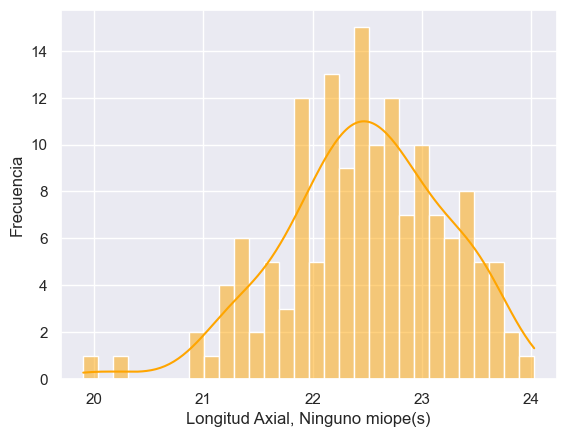
\includegraphics[height=.95\linewidth, width=.95\linewidth]{assets/AL_none_hist}
%				\caption{}
%				\label{fig:5b}
%			\end{subfigure}
%			\begin{subfigure}{.49\linewidth}
%				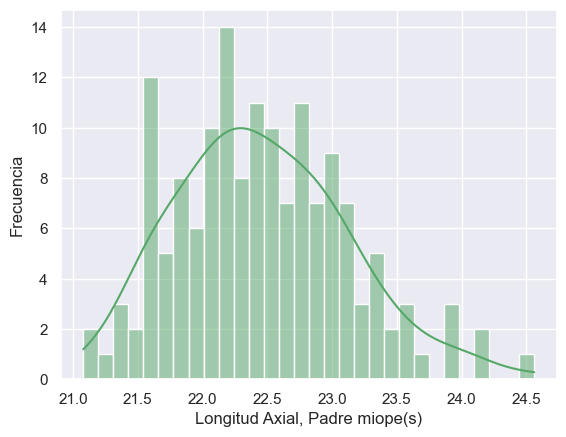
\includegraphics[height=.95\linewidth, width=.95\linewidth]{assets/AL_dad_hist}
%				\caption{}
%				\label{fig:5c}
%			\end{subfigure}
%			\begin{subfigure}{.49\linewidth}
%				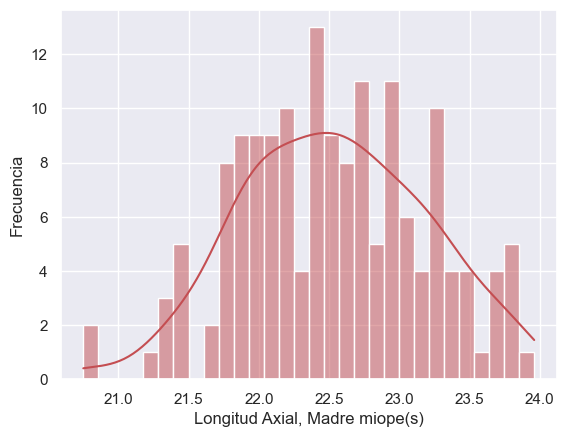
\includegraphics[height=.95\linewidth, width=.95\linewidth]{assets/AL_mom_hist}
%				\caption{}
%				\label{fig:5d}
%			\end{subfigure}
%			\caption{La distribución de la Longitud Axial en cada uno de los grupos de intrés (usando histogramas y estimación de densidad). }
%			\label{fig:5}
%		\end{figure}
%		
%		\begin{figure}[htb]%
%			\begin{center}
%				\centering
%				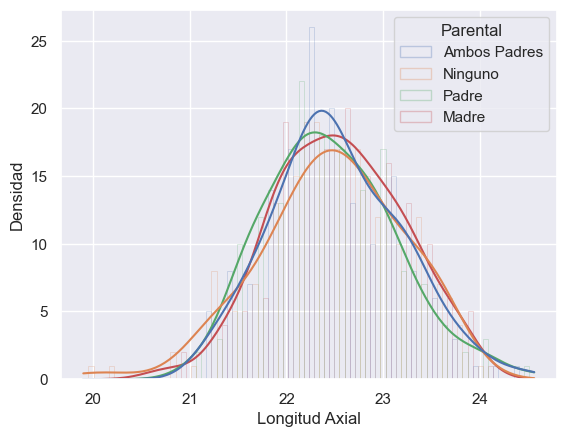
\includegraphics[height = .75\linewidth, width=.75\linewidth]{assets/AL_groups_kde}
%			\end{center}
%			\caption{Comparación de la distribución de cada grupo (según la información parental).}
%			\label{fig:3}
%		\end{figure}
	
	
%-----------------------------------------------------------------------------------
%	\subsection{Listas y Descripciones}\label{sub:lists}
%%-----------------------------------------------------------------------------------
%		Para producir listas enumeradas, utilice el siguiente estilo:
%		\begin{enumerate}
%			\item Primer Elemento
%			\item Segundo Elemento
%			%
%			\begin {enumerate}
%				\item {Segundo Elemento - Subítem Uno}
%				\item {Segundo Elemento - Subítem Dos}
%			\end {enumerate}
%			%
%		\end{enumerate}
%
%%-----------------------------------------------------------------------------------
%		Para producir descripciones, use el siguiente estilo:
%
%%-----------------------------------------------------------------------------------
%		\begin{description}
%			\item [Primer Elemento] con su respectiva descripción.
%			\item [Segundo Elemento] también con su respectiva descripción.
%		\end{description}


%%-----------------------------------------------------------------------------------
%	\subsection{Código Fuente}\label{sub:listings}
%%-----------------------------------------------------------------------------------
%		Para producir código fuente, envuélvalo en una figura flotante y
%		etiquételo correctamente. Por ejemplo, en la Fig. \ref{fig:code}
%		se muestra un código bastante conocido\ldots
%
%		% Configuración de Listings
%		\lstset{keywordstyle=\color{blue}, basicstyle=\small}
%
%		\begin{figure}[htb]%
%			\begin{lstlisting}[language=c]%
%
%    int main(int argc, char** argv)
%    {
%        // Imprimiendo "Hola Mundo".
%        printf("Hello, World");
%    }
%
%			\end{lstlisting}
%		\caption{Código fuente de ejemplo.\label{fig:code}}
%		\end{figure}

%%-----------------------------------------------------------------------------------
%	\subsection{Referencias}
%%-----------------------------------------------------------------------------------
%  	Las referencias deben estar agrupadas en una sección al final del artículo,
%  	y las citas numeradas correctamente, por ejemplo \cite{knuth} o \cite{goedel}.
%  	Incluya toda la información importante de cada referencia, incluídos autor,
%  	título, y notas de la edición. En caso de citar sitios web, además
%  	de la URL, incluya la fecha en que fue consultado, como en \cite{wiki}. Numere 
%  	las referencias según el orden en que se les cita.

%===================================================================================



%===================================================================================
% Conclusiones
%-----------------------------------------------------------------------------------
\section{Conclusiones}\label{sec:conc}

%  Se probó que, aunque el factor genético pueda influenciar la miopía, no existe evidencia suficiente para afirmar que la presencia de la enfermedad en los padres influencia notoriamente en la anatomía de los ojos de la decendencia a tempranas edades. Se comprobó además que la AL sigue una distribución normal, y que efectivamente factores étnicos son definitorios en el tamaño del globo ocular, y por tanto puede ser determinante en el riesgo de aparición de la enfermedad. Sentando con todos estos elementos, las bases para un posterior análisis predictivo de la enfermedad a edades tempranas.

%===================================================================================



%===================================================================================
% Recomendaciones
%-----------------------------------------------------------------------------------
\section{Recomendaciones}\label{sec:rec}

% Probadas las capacidades de las herramientas convencionales para el análisis de datos en este campo tan importante de la medicina, se recomienda realizar un estudio de este tipo sobre la Miopía en Cuba, teniendo en cuenta los factores étnicos que componen su sociedad. Debe tenerse en cuenta que la cantidad de pacientes diagnosticados con miopía, a pesar de ser lo suficientemente grande para plantear pruebas de hipótesis, es considerablemente baja teniendo en cuenta los pacientes emétropes; lo cual puede afectar cosiderablemente la precisión de cualquier modelo predictivo que se formule con los datos, siendo estos propensos a errores de tipo 2, falsos negativos, diagnóstico erróneo en pacientes enfermos.

%===================================================================================



%===================================================================================
% Bibliografía
%-----------------------------------------------------------------------------------
\begin{thebibliography}{99}
%-----------------------------------------------------------------------------------

	
%	====================== REFERENCES======================================
	
	\bibitem{batlle}
	Batlle Almodóvar MC, Dickinson Meneses FO. Revista Habanera de Ciencias Médicas \textit{Historia de la meningitis bacteriana en Cuba: siglo XIX al XXI. }. 2019;18(4):579-592.  \href{https://revhabanera.sld.cu/index.php/rhab/article/view/2972/2387.}{https://revhabanera.sld.cu/}
	
	\bibitem{GBD2021}
	Global Burden of Disease Collaborative Network. (2022). \textit{Global Burden of Disease Study 2021 (GBD 2021) Results}. Seattle, United States: Institute for Health Metrics and Evaluation (IHME). Disponible en \href{https://vizhub.healthdata.org/gbd-results/}{https://vizhub.healthdata.org/}
	
	\bibitem{Jung2018}
	Jung, S., Lee, H., \& Nishiura, H. (2018). \textit{The impact of pneumococcal vaccination on pneumonia mortality among the elderly in Japan: a difference-in-difference study}
	\href{https://doi.org/10.7717/peerj.6085}{DOI 10.1146/peerj.6085.}
	
	
	\bibitem{OMS_meinigitis}
	Organización Mundial de la Salud. (2023). \textit{Meningitis}. Recuperado de 	\href{https://www.who.int/es/news-room/fact-sheets/detail/meningitis}{https://www.who.int/es}
	
	\bibitem{valcarcel}
	Valcárcel M, Rodríguez CR, Molinert HT. \textit{La enfermedad meningocóccica en Cuba: cronología de una epidemia}. La Habana: Editorial Ciencias Médicas; 1991.
	
	\bibitem{wing} Wing C, Simon K, Bello-Gomez RA. (2018). \textit{Designing difference in difference studies: best practices for public health policy research. Annual Review of Public Health 39(1):453–469  } 
	\href{http://dx.doi.org/10.1146/annurev-publhealth-040617-013507}{DOI 10.1146/annurev-publhealth-040617-013507.}
	
	
	
	
%	\bibitem{knuth} Donald E. Knuth. \emph{The Art of Computer Programming}.
%		Volume 1: Fundamental Algorithms (3rd~edition), 1997.
%		Addison-Wesley Professional.
%
%	\bibitem{goedel} Kurt Göedel. \emph{Über formal unentscheidbare Sätze der
%		Principia Mathematica und verwandter Systeme, I}.
%		Monatshefte für Mathematik und Physik 38.
%
%	\bibitem{wiki} Wikipedia. URL: \href{http://en.wikipedia.org}
%	  {http://en.wikipedia.org}.
%		Consultado en \today.

%-----------------------------------------------------------------------------------
\end{thebibliography}

%-----------------------------------------------------------------------------------

\label{end}

\end{document}

%===================================================================================
